\PassOptionsToPackage{hyphens}{url}
\documentclass[compress,aspectratio=169]{beamer}

\usetheme{Reading}

\graphicspath{{../2019-06-isc/}{../2019-06-isc/fig/}{img/}{../logo/}}

\newcommand{\ok}[1]{{#1 (done)}}
\newcommand{\ongoing}[1]{{#1 (ongoing)}}
\newcommand{\started}[1]{{#1 (started)}}
\newcommand{\pending}[1]{{#1 (pending in plan)}}
\newcommand{\hrefb}[2]{\href{#1}{\textcolor{blue}{#2}}}

\subtitle{}
\title{\Large Contributing HPC Skills to the HPC Certification Forum}
\author{J. Kunkel, Kai Himstedt, Weronika Filinger, Jean-Thomas Acquaviva, Anja Gerbes, Lev Lafayette}
\date{2019-11-17}
\authorURL{https://hpc-certification.org}
\authorFooter{Julian M. Kunkel et al.}
\venue{BPHTE19 Workshop}
\institute{Department of Computer Science}
\groupLogo{
\includegraphics[width=2.5cm]{hpccf-small}}
\titleLogo{ 
\includegraphics[height=2.5cm]{blur-book-stack-books-590493}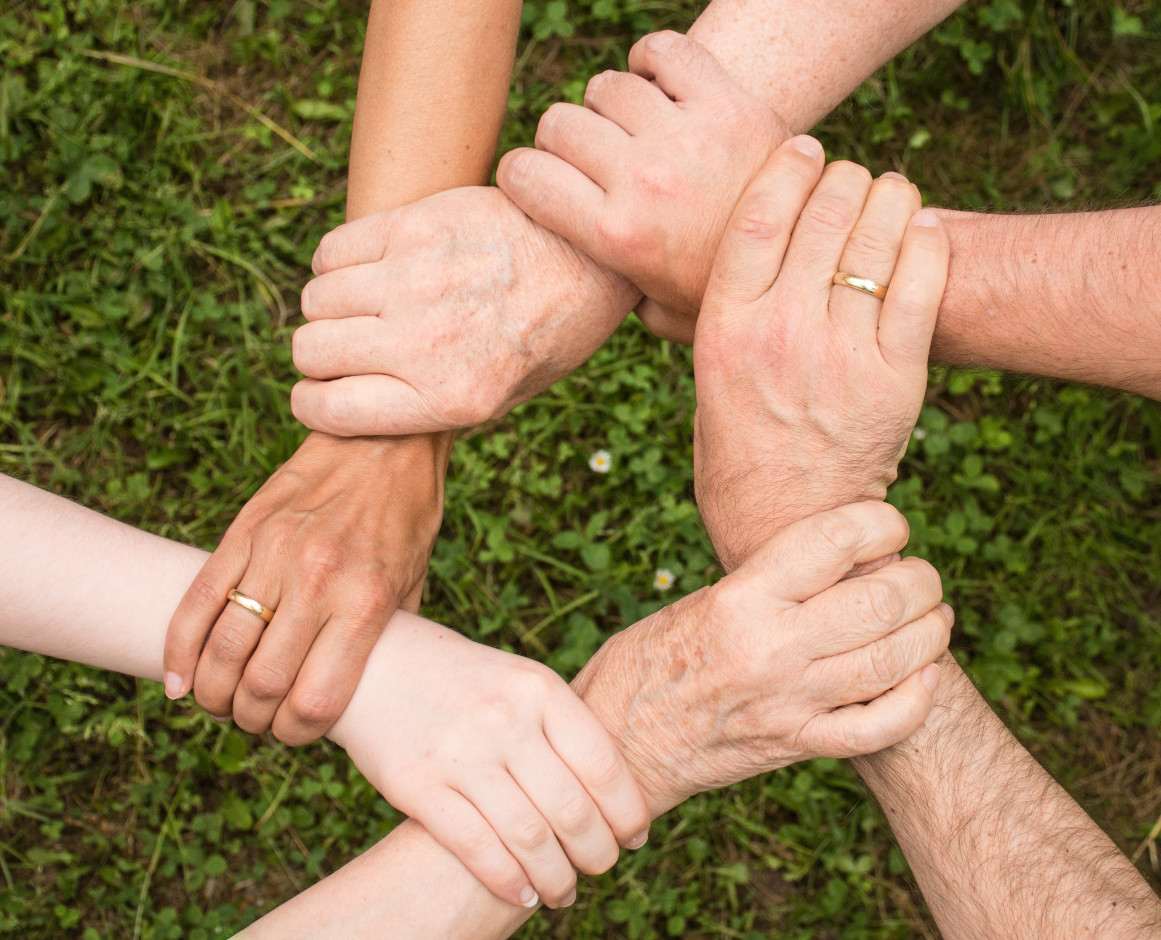
\includegraphics[height=2.5cm]{ground-group-growth-461049}
\includegraphics[height=2.5cm]{accomplishment-ceremony-college-267885}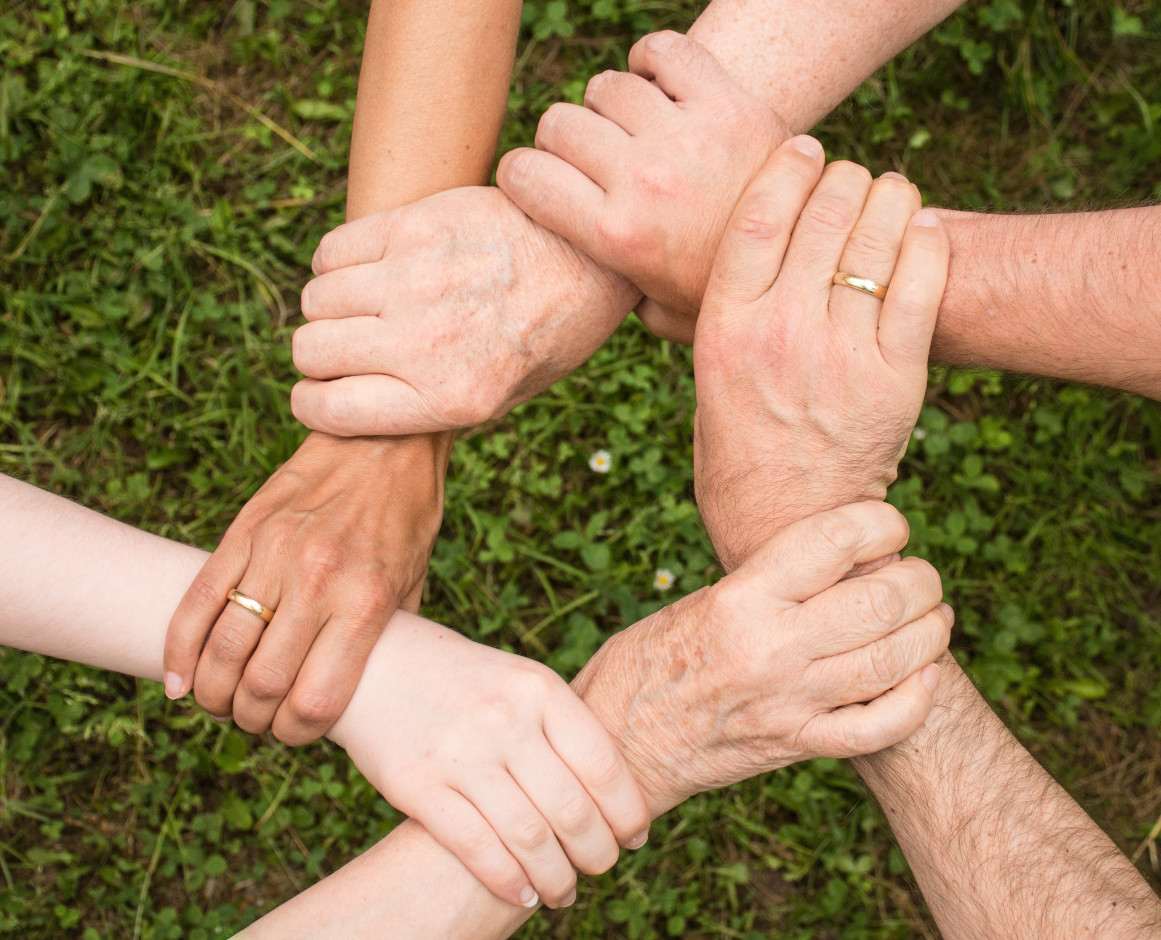
\includegraphics[height=2.5cm]{ground-group-growth-461049}
\includegraphics[height=2.5cm]{blur-book-stack-books-2}}


\begin{document}

\begin{frame}[plain]{}
	\maketitle
	{\fontsize{5.85pt}{6pt}\selectfont PeCoH is supported by Deutsche Forschungsgemeinschaft (DFG) under grants LU 1335/12-1, OL 241/2-1, RI 1068/7-1}
\end{frame}


%       the nature of the training or education program
%       Strategy
%       assessment or evaluation technique
%       situations for which it is relevant or in which it was applied
%       an evaluation of its success
%       lessons learned
%       reproducibility of the processes and resources

\section{The Program}
\sectionIntroHidden

\subsection{}

\begin{frame}{The HPC Certification Program}
		\begin{block}{Goals}
			\begin{itemize}
				\item Fine-grained standardizing HPC knowledge representation
          \begin{itemize}
            \item What competences exist, how are they defined?
            \item Puzzle of competences for everyone (practitioners, students)
            \item Supporting navigation and role-specific knowledge maps
          \end{itemize}
				\item Establishing international certificates attesting knowledge
			\end{itemize}
		\end{block}

		\begin{block}{Important!}
			\begin{itemize}
				\item We do not compete with content providers
				\item We do not intent to create a curriculum
			\end{itemize}
		\end{block}

    \begin{block}{This talk is about contributing to the knowledge representation}
    \end{block}
\end{frame}


\begin{frame}{The 
\includegraphics[width=0.45\textwidth]{hpccf-full}}
	The HPC-CF is the central authority for the development of the program

	\begin{block}{Organization Details}
		\begin{itemize}
			\item An independent international body
			\item Organized into
				\begin{itemize}
					\item Steering board
					\item Full members with voting rights
					\item Associate members
          \item Collaboration with e.g., SIGHPC Education Chapter
				\end{itemize}
		\end{itemize}
	\end{block}

	\begin{block}{Responsibilities}
		\begin{itemize}
			\item Curating and maintaining the skill tree and certificates
			\item Providing tools and ecosystem around the competences
		\end{itemize}
	\end{block}
\end{frame}

\begin{frame}{Example High-Level Skill}

\begin{itemize}
\item Name: SLURM Workload manager
\item Id: USE4.2.2-B
\item Background: {\small SLURM is a widely used open-source workload
manager providing various advanced features.}
\item Aim:
\begin{itemize}
\item comprehend and describe the basic architecture of SLURM and its tools
\item use relevant tools to run and monitor (parallel) applications
\end{itemize}
\end{itemize}

\begin{block}{Learning outcomes}
\begin{itemize}
\item run interactive jobs with salloc, a batch job with sbatch
\item explain the architecture of SLURM, i.e., the role of slurmd, srun
\item explain the function of the tools: sacct, sbatch, salloc, ...
\item explain time limits and the benefit of a backfill scheduler
\item see \url{https://www.hpc-certification.org/wiki/}
\end{itemize}
\end{block}
\end{frame}


\begin{frame}{Content of the Certification Program}
	\begin{itemize}
		\item A \textbf{skill} defines background, objectives, learning outcomes
		\item The \textbf{skill tree} organizes the competences as hierarchical skills
		\item Certificates bundle several skills into attestable unit
	\end{itemize}

	\begin{figure}
		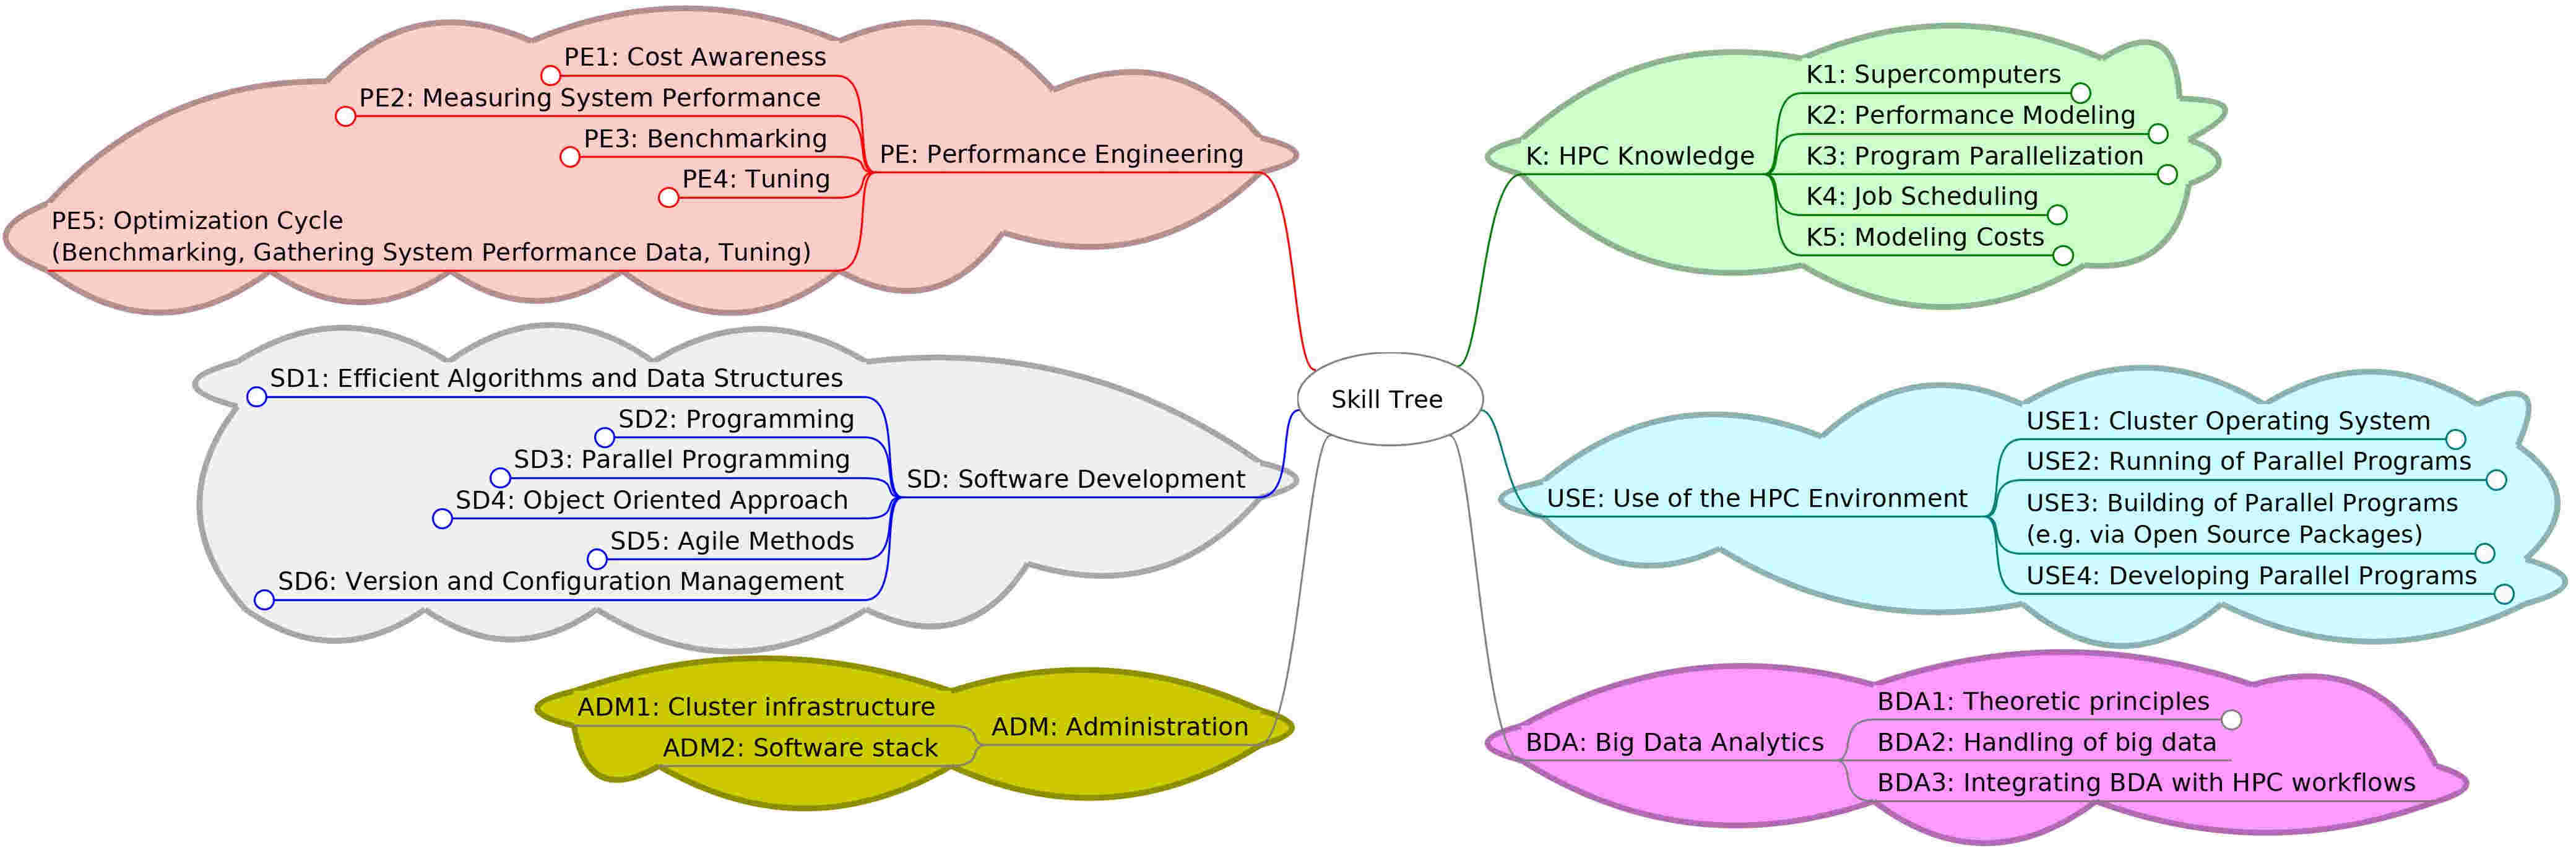
\includegraphics[width=\textwidth]{skill-tree}
		\vspace*{-2em}
		\caption{Top-levels of the skill tree (We are working on ADM and BDA branches)}
	\end{figure}
\end{frame}

\section{Contributing}

\begin{frame}{High-Level Editing}
  \begin{itemize}
    \item Webpage with Markdown version controlled in Git
      \begin{itemize}
        \item \url{https://www.hpc-certification.org/wiki/skill-tree/b}
        \item GitHub: \url{https://github.com/HPC-certification-forum/skill-tree}
      \end{itemize}
    \item Editing a MindMap, the structure of Skills
      \begin{itemize}
        \item Synchronized with the skill tree in Git
        \item Uses the OpenSource tool Freemind
      \end{itemize}
    \item Discussion on our \href{https://join.slack.com/t/hpc-certification/shared_invite/enQtMzUwNzU3NzM2MTkzLTAzZWM3NDg0N2I2ZmQwOWI5ZGUwNjNlNDgzM2RmOTM3ZWRjNjIxYTc5NzUxYTJhNmRlNmM5YmE1NDY3YzkzYzA}{Slack}
    \item We welcome any contribution via either channel
      \begin{itemize}
        \item Pull requests are also welcome
      \end{itemize}
  \end{itemize}
\end{frame}

\begin{frame}{Webpage}
  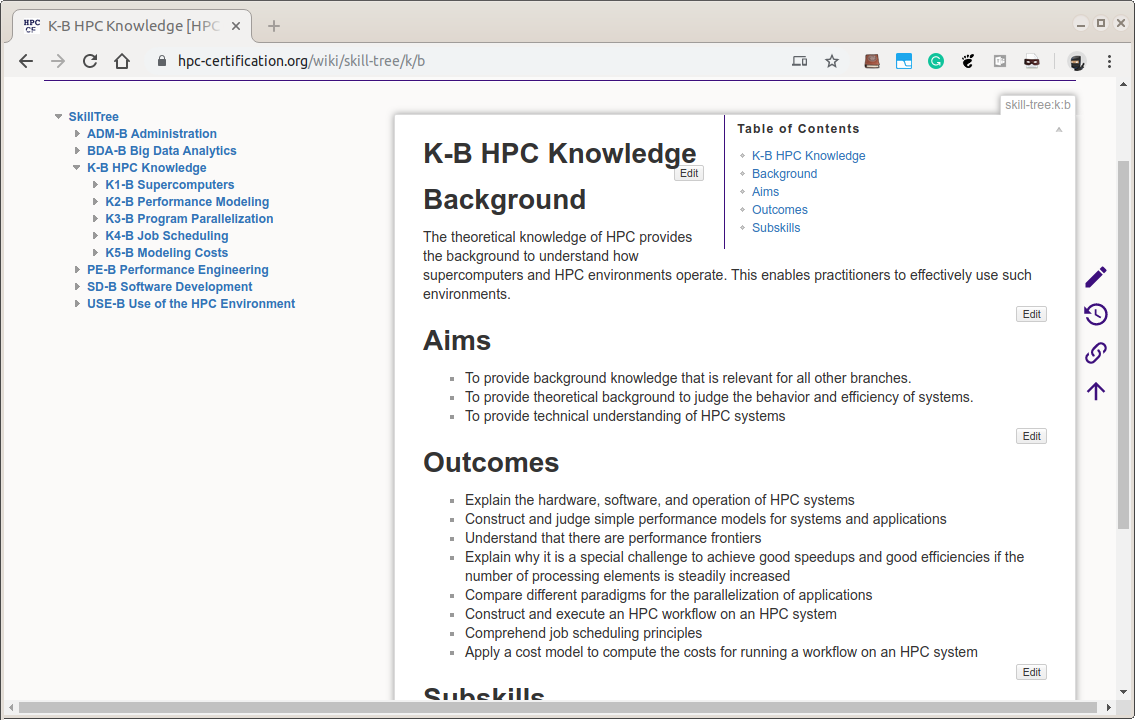
\includegraphics[width=0.8\textwidth]{www}
\end{frame}


\end{document}
